\chapter{Results and Statistical Validation}\label{ch:results}

This chapter reports the fixed temporal holdout experiment saved by the final
experiment artifact. The reported values match that artifact. The evaluation is
not a new-patient external validation. It is a patient-adapted temporal test:
earlier MLII ECG from each eligible MITDB record is available during training
and selection, and only the final 20\% timeline is scored as unseen signal from
the same known patients.

\section{What was tested}

Figure~\ref{fig:final-testing-protocol} summarises the actual final test. The
test data came only from the MIT--BIH Arrhythmia Database. Records 102 and 104
were excluded because they do not contain MLII. The remaining 46 records with
MLII represent 45 subject clusters, with records 201 and 202 treated as one
subject. No NSRDB beat is part of the final temporal test. NSRDB contributes
only the already frozen normal autoencoder, which creates four residual
features for each MITDB MLII beat.

\begin{figure}[H]
\centering
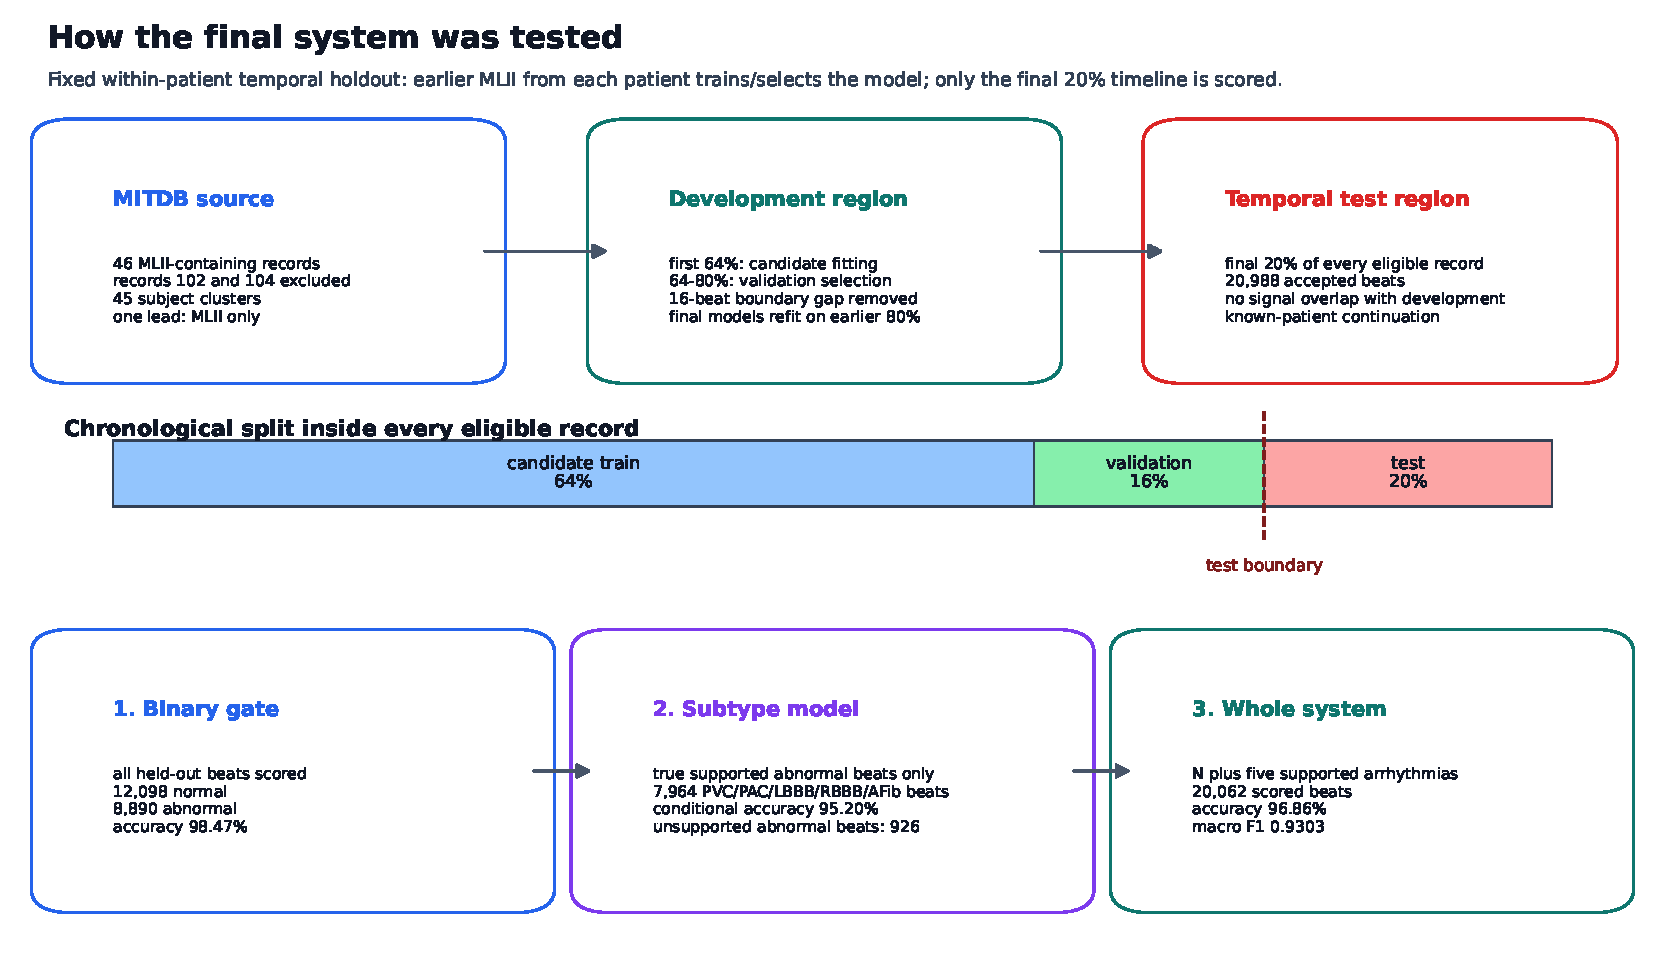
\includegraphics[width=.98\textwidth]{pic/generated/final_testing_protocol.pdf}
\caption{Final testing protocol. Each eligible MITDB MLII record is split in
time. Candidate fitting and validation use only earlier beats; the final 20\%
timeline is held out for scoring.}
\label{fig:final-testing-protocol}
\end{figure}

\begin{table}[H]
\centering
\caption{Data used by each final evaluation.}
\label{tab:final-test-data}
\begin{tabular}{>{\raggedright\arraybackslash}p{.25\textwidth}
                >{\raggedright\arraybackslash}p{.24\textwidth}
                >{\raggedright\arraybackslash}p{.42\textwidth}}
\toprule
Evaluation & Test support & Meaning\\
\midrule
Binary abnormality detection & 20,988 held-out beats:
12,098 normal and 8,890 abnormal & Tests whether the gate separates normal
from abnormal. Unsupported abnormal MITDB symbols are included here because
they are still abnormal beats.\\
Conditional subtype classification & 7,964 supported abnormal beats & Tests
the subtype model only on true PVC, PAC, LBBB, RBBB, and AFib beats. This
ignores the binary gate so subtype naming can be inspected separately.\\
Whole-system six-class output & 20,062 supported beats & Tests the deployed
hierarchy after the binary gate: N/PVC/PAC/LBBB/RBBB/AFib. The 926 unsupported
abnormal beats are not included in the six-class confusion matrix.\\
\bottomrule
\end{tabular}
\end{table}

\begin{figure}[H]
\centering
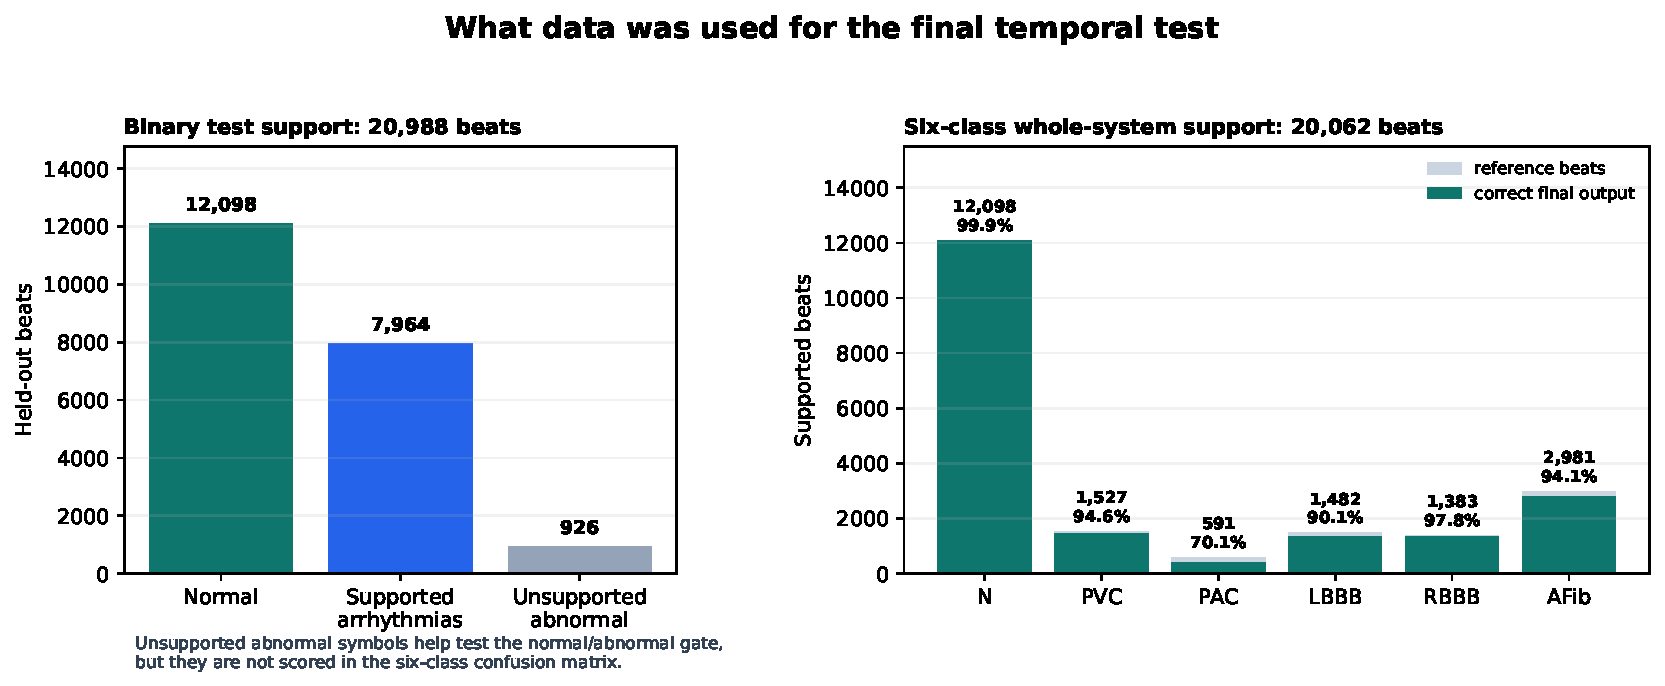
\includegraphics[width=.98\textwidth]{pic/generated/final_test_composition.pdf}
\caption{Composition of the held-out temporal test data. The binary test uses
all accepted held-out beats. The six-class whole-system test uses normal beats
and the five supported abnormal classes.}
\label{fig:final-test-composition}
\end{figure}

\section{Model selection before final testing}

In this rerun, the final 20\% segment did not choose the model or the
threshold. Candidate selection used the 64--80\% validation region. The
selected binary model was a fully grown 240-tree Extra Trees ensemble using
square-root feature sampling, leaf size one, and record-weighting power 0.35.
Its selected abnormal threshold was 0.6208333, and its validation balanced
accuracy was 98.90\%. The selected subtype model was a fully grown 260-tree
ensemble using one-third feature sampling, leaf size one, and record-weighting
power 0.25. Its validation macro F1 was 0.9803. After selection, both
supervised models were refitted on the earlier 80\% development region,
excluding the 16-beat boundary gap before the temporal test.

\section{Headline temporal performance}

\begin{table}[H]
\centering
\caption{Final temporal results. Confidence intervals use equal-subject scores,
not pooled beats.}
\label{tab:final-headline}
\begin{tabular}{lrrrr}
\toprule
Outcome & Pooled score & Subject-macro & 95\% CI & Width\\
\midrule
Abnormality accuracy & 98.47\% & 98.53\% & 97.16--99.41\% & 2.26 pp\\
Conditional subtype accuracy & 95.20\% & 93.80\% & 87.71--98.58\% & 10.86 pp\\
Whole-system accuracy & 96.86\% & 96.90\% & 94.02--99.05\% & 5.03 pp\\
\bottomrule
\end{tabular}
\end{table}

The binary gate reached 98.47\% pooled accuracy, 98.22\% balanced accuracy,
96.59\% sensitivity, 99.85\% specificity, 99.79\% precision, and binary F1 of
0.9817. Conditional subtype accuracy on true supported abnormal beats was
95.20\%, with macro F1 of 0.9325. After the gate and subtype model were
combined, whole-system six-class accuracy was 96.86\% and macro F1 was 0.9303.

\begin{figure}[H]
\centering
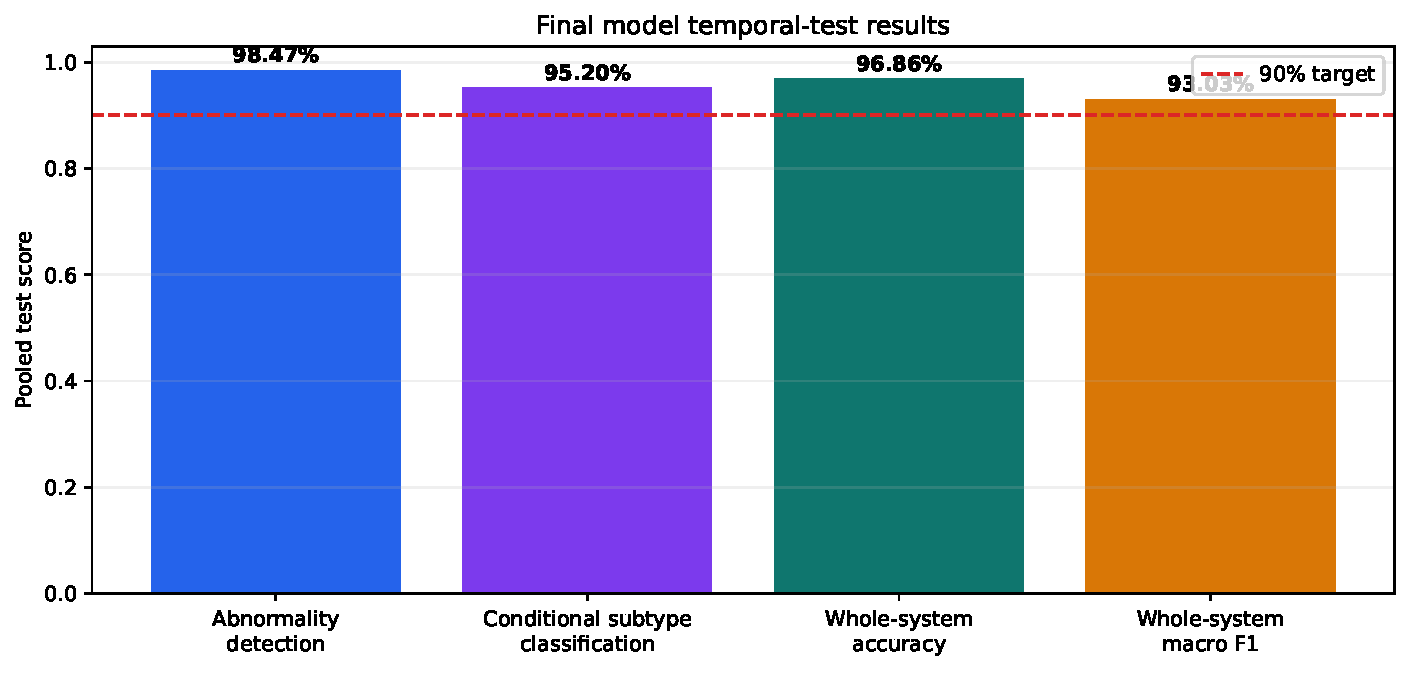
\includegraphics[width=.96\textwidth]{pic/generated/final_metrics.pdf}
\caption{Pooled temporal-test results. Binary accuracy, conditional subtype
accuracy, whole-system accuracy, and whole-system macro F1 are all above
90\%.}
\label{fig:final-metrics}
\end{figure}

The primary point estimate exceeded the 90\% target, and the lower bound of the
equal-subject 95\% confidence interval was also above 90\%. The complete
planned statistical goal was not fully met because the whole-system confidence
interval was 5.03 percentage points wide. The planned maximum was three
percentage points.

\section{Subject-clustered validation}

The statistical validation treats subjects, not beats, as the independent
units. Each bootstrap replicate sampled complete subject clusters with
replacement, kept records 201 and 202 inside one subject cluster, and then
calculated equal-subject accuracy. This prevents the 20,988 related beats from
making the confidence interval falsely narrow.

\begin{figure}[H]
\centering
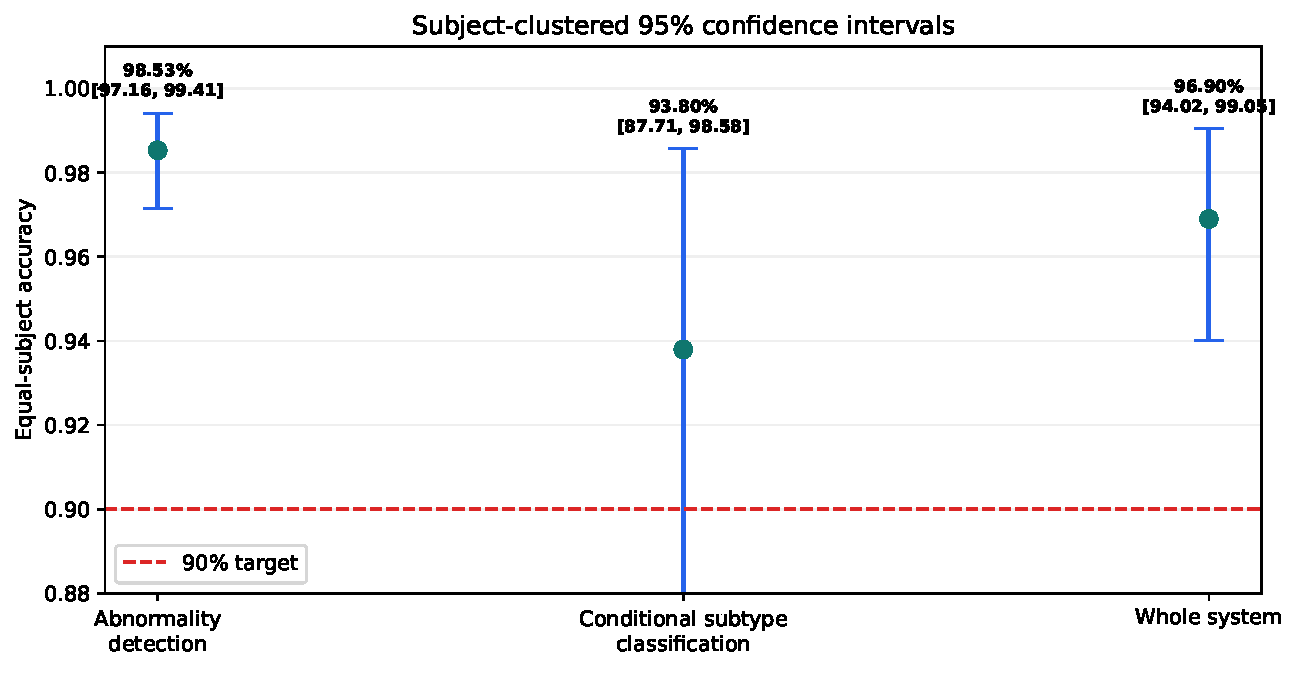
\includegraphics[width=.90\textwidth]{pic/generated/final_clustered_ci.pdf}
\caption[Subject-clustered confidence intervals.]{Equal-subject estimates and 95\% subject-cluster bootstrap intervals.
The whole-system lower bound remains above 90\%, but the interval width is
larger than planned.}
\label{fig:final-ci}
\end{figure}

Forty-two of 45 subject clusters had whole-system accuracy above 90\%. The
exact one-sided sign test gave $p=4.33\times10^{-10}$ for the hypothesis that
more than half of subjects exceed 90\%. A secondary one-sided Wilcoxon
signed-rank test gave statistic 903 and $p=5.63\times10^{-6}$ for a positive
shift above 90\%. These tests support the conclusion that performance is above
90\% for this known-patient temporal problem, but the confidence interval
remains the primary effect-size evidence.

\begin{figure}[H]
\centering
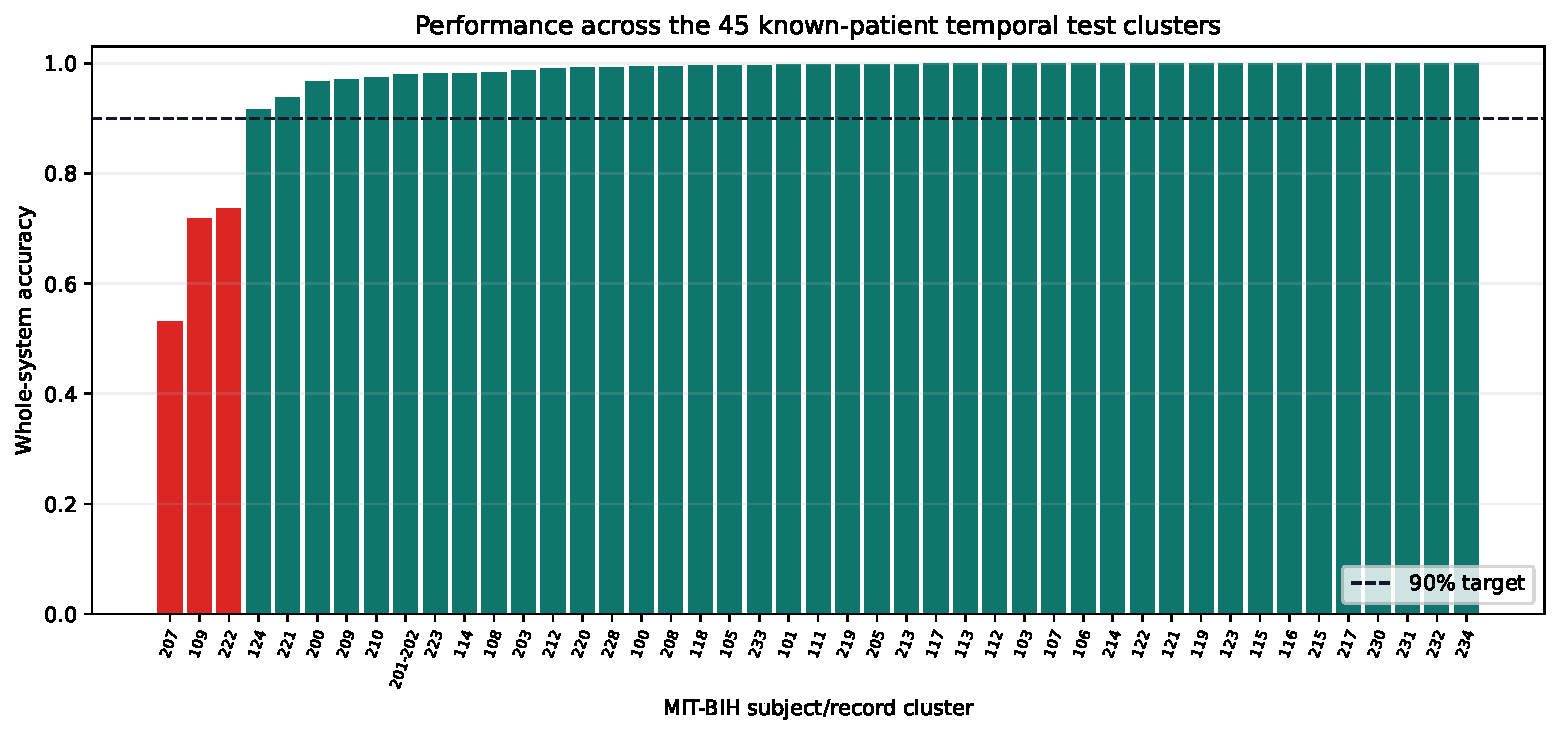
\includegraphics[width=.98\textwidth]{pic/generated/final_subject_accuracy.pdf}
\caption{Whole-system accuracy for all 45 subject clusters. Red bars are below
90\%; 42 clusters are above the target.}
\label{fig:final-subjects}
\end{figure}

The below-target clusters were 207 (53.10\%), 109 (71.74\%), and 222
(73.59\%). Cluster 207 mainly reflects subtype confusion, while cluster 222 has
a weaker binary result. The next-lowest cluster, 124, reached 91.64\%. This
subject variation explains why the equal-subject confidence interval is much
wider than a pooled beat-level summary would suggest.

\section{Stage-by-stage results}

The binary gate was tested on all 20,988 held-out beats. It correctly detected
8,587 of 8,890 abnormal beats and correctly rejected 12,080 of 12,098 normal
beats. The remaining binary errors were 303 missed abnormal beats and 18 false
alarms. This stage meets the aggregate accuracy, lower-bound, and interval
width targets.

The subtype model was evaluated independently on 7,964 true supported abnormal
beats. It correctly named 95.20\% of them before the binary gate was applied.
This explains why the conditional subtype score is higher than the final
end-to-end subtype recall for some arrhythmias. A beat can be named correctly
by the subtype model but still be sent to normal by the binary gate.

\section{Results for each arrhythmia}

\begin{table}[H]
\centering
\caption{End-to-end class performance on real labeled temporal test beats.}
\label{tab:final-arrhythmias}
\begin{tabular}{lrrrrrr}
\toprule
Type & True & Correct & Precision & Recall & F1 & 90\% recall\\
\midrule
PVC  & 1,527 & 1,445 & 85.30\% & 94.63\% & 0.8972 & Reached\\
PAC  & 591   & 414   & 98.57\% & 70.05\% & 0.8190 & Not reached\\
LBBB & 1,482 & 1,336 & 95.09\% & 90.15\% & 0.9255 & Reached\\
RBBB & 1,383 & 1,352 & 99.78\% & 97.76\% & 0.9876 & Reached\\
AFib & 2,981 & 2,806 & 98.77\% & 94.13\% & 0.9639 & Reached\\
\bottomrule
\end{tabular}
\end{table}

\begin{figure}[H]
\centering
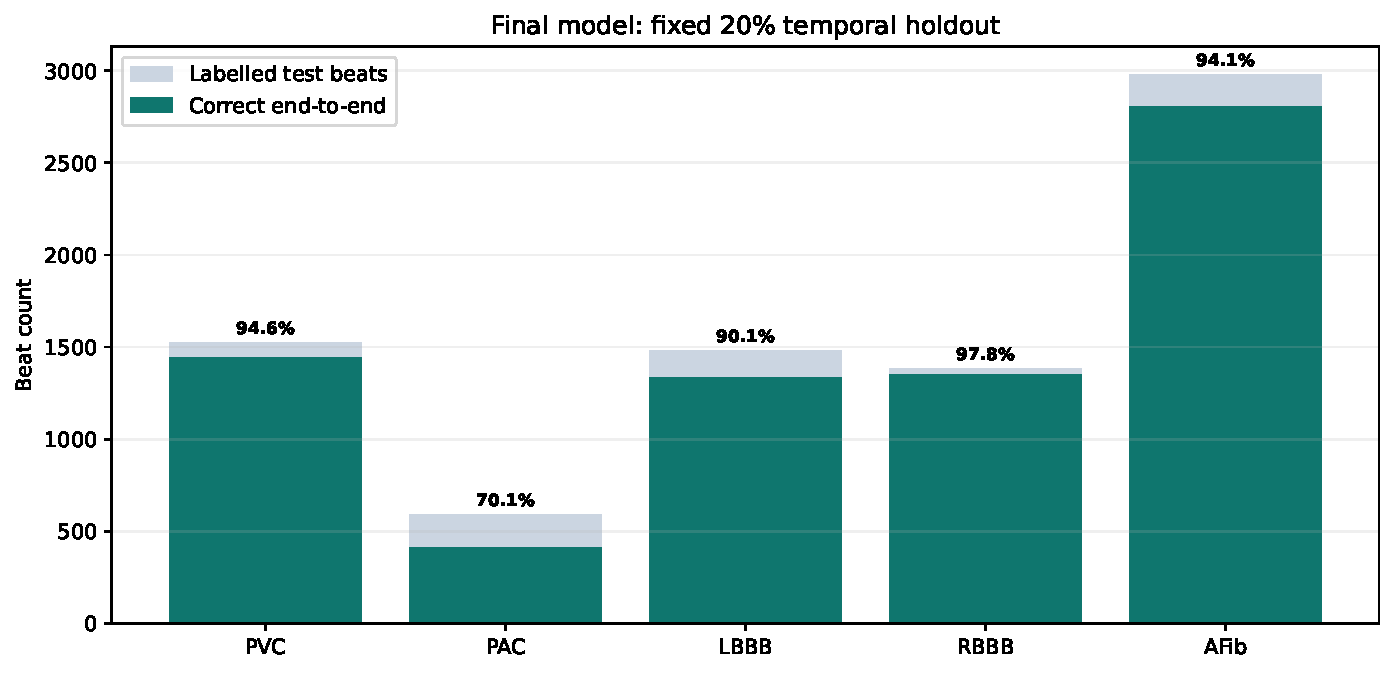
\includegraphics[width=.95\textwidth]{pic/generated/final_arrhythmia_counts.pdf}
\caption{Reference and correctly classified arrhythmia counts. PAC is the only
supported abnormal class with end-to-end recall far below 90\%.}
\label{fig:final-arrhythmia-counts}
\end{figure}

PVC, LBBB, RBBB, and AFib exceeded 90\% end-to-end recall. PAC did not. Of 591
PAC beats, the binary detector marked 540 abnormal, the independent subtype
model named 445 correctly before gating, and only 414 survived both decisions
with the correct final output. Therefore, PAC loss comes from both the binary
gate and the subtype model, with subtype confusion contributing more. The
aggregate system accuracy must not be interpreted as equal strength for every
arrhythmia.

\section{Whole-system confusion matrix}

\begin{figure}[H]
\centering
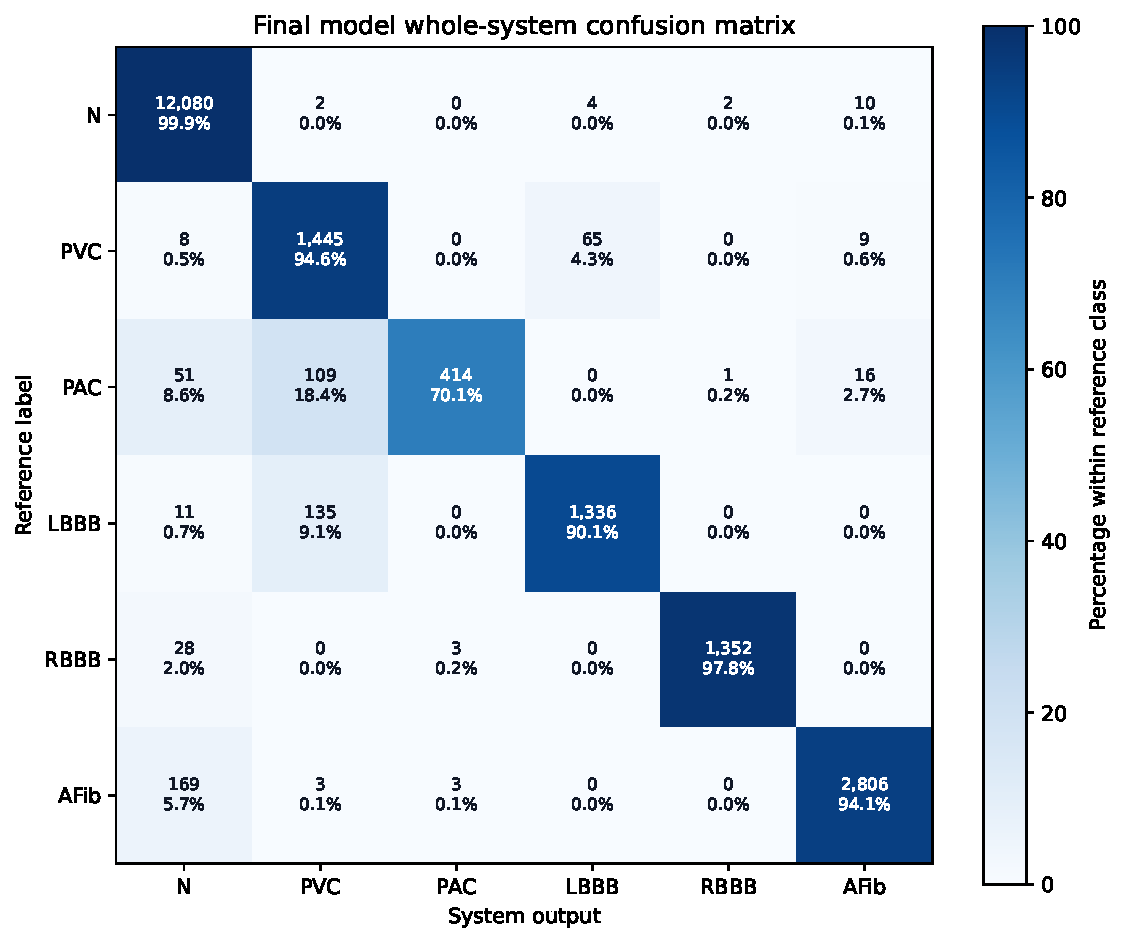
\includegraphics[width=.86\textwidth]{pic/generated/final_confusion_matrix.pdf}
\caption{Confusion matrix for 20,062 supported temporal-test beats. Counts and
row percentages are shown together.}
\label{fig:final-confusion}
\end{figure}

The diagonal dominates the confusion matrix, but the remaining errors show the
main failure modes. The largest subtype confusions are 135 LBBB beats assigned
to PVC, 109 PAC beats assigned to PVC, and 65 PVC beats assigned to LBBB. The
binary gate sends 169 AFib beats and 51 PAC beats to normal. These errors are
clinically important even though the aggregate whole-system accuracy is high.

\section{Interpretation of the temporal result}

The final result should be read as evidence for temporal continuation after
patient exposure. Earlier ECG from the same patient provides morphology, lead
orientation, and rhythm context that can make later beats easier to classify.
The chronological boundary and 16-beat gap prevent direct signal overlap, but
they do not remove patient identity. Therefore, the 96.86\% whole-system
accuracy is valid for known-patient temporal holdout performance. It is not
proof of cold-start performance on completely unseen patients.

\section{External INCART unseen-dataset check}\label{sec:external-incart}

After the final MITDB temporal-holdout system had been fixed, a separate
external check was run on the St Petersburg INCART 12-lead Arrhythmia Database.
This is not the primary thesis benchmark and it is not used for model
selection. It is included to show how the frozen system behaves on an unseen
source database with a different acquisition setting. Lead II is used because
it is the closest practical counterpart to MITDB MLII, but it is not identical
to MLII. Therefore, this section measures both external-patient shift and
lead/device-domain shift.

\begin{figure}[H]
\centering
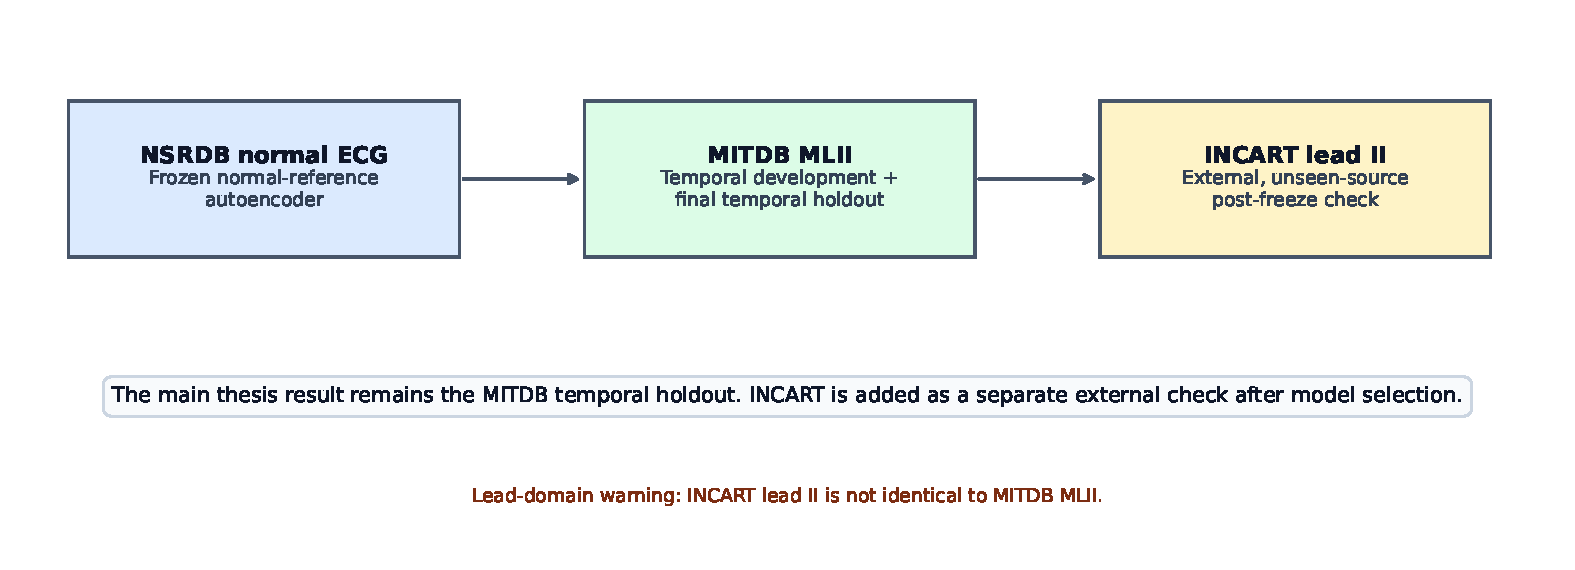
\includegraphics[width=.98\textwidth]{pic/generated/external_incart_protocol.pdf}
\caption{Separation between the main MITDB temporal result and the INCART
external check. The external result is reported after model selection and is
not used to tune the frozen system.}
\label{fig:external-incart-protocol}
\end{figure}

\begin{table}[H]
\centering
\caption{Limited external INCART check on the latest saved evaluation artifact.}
\label{tab:external-incart-summary}
\begin{tabular}{ll}
\toprule
Item & Value\\
\midrule
Dataset & St Petersburg INCART 12-lead Arrhythmia Database\\
Lead and mode & II, offline\\
Records scored & 1 (I01)\\
Annotated beats & 120\\
Saved artifact time & 2026-08-24T09:45:26.627767+00:00\\
Decision threshold & 0.6208\\
Accuracy & 98.33\%\\
Balanced accuracy & 99.10\%\\
Sensitivity / specificity & 100.00\% / 98.20\%\\
Precision / F1 & 81.82\% / 90.00\%\\
AUROC / AUPRC & 1.0000 / 1.0000\\
Confusion counts & TP=9, TN=109, FP=2, FN=0\\
Subtype macro F1 & 0.9691\\
\bottomrule
\end{tabular}
\end{table}

On this limited INCART subset, the frozen hierarchy reached 98.33\%
binary accuracy and 99.10\% balanced accuracy.
All 9 annotated abnormal beats in the subset were detected
and 109 normal beats were rejected, while 2
normal beats were false alarms and 0 abnormal beats were
missed. Because the subset is small and contains only 120
accepted beats from 1 INCART record, this result should be read
as an external sanity check, not as a definitive external clinical validation.

\begin{figure}[H]
\centering
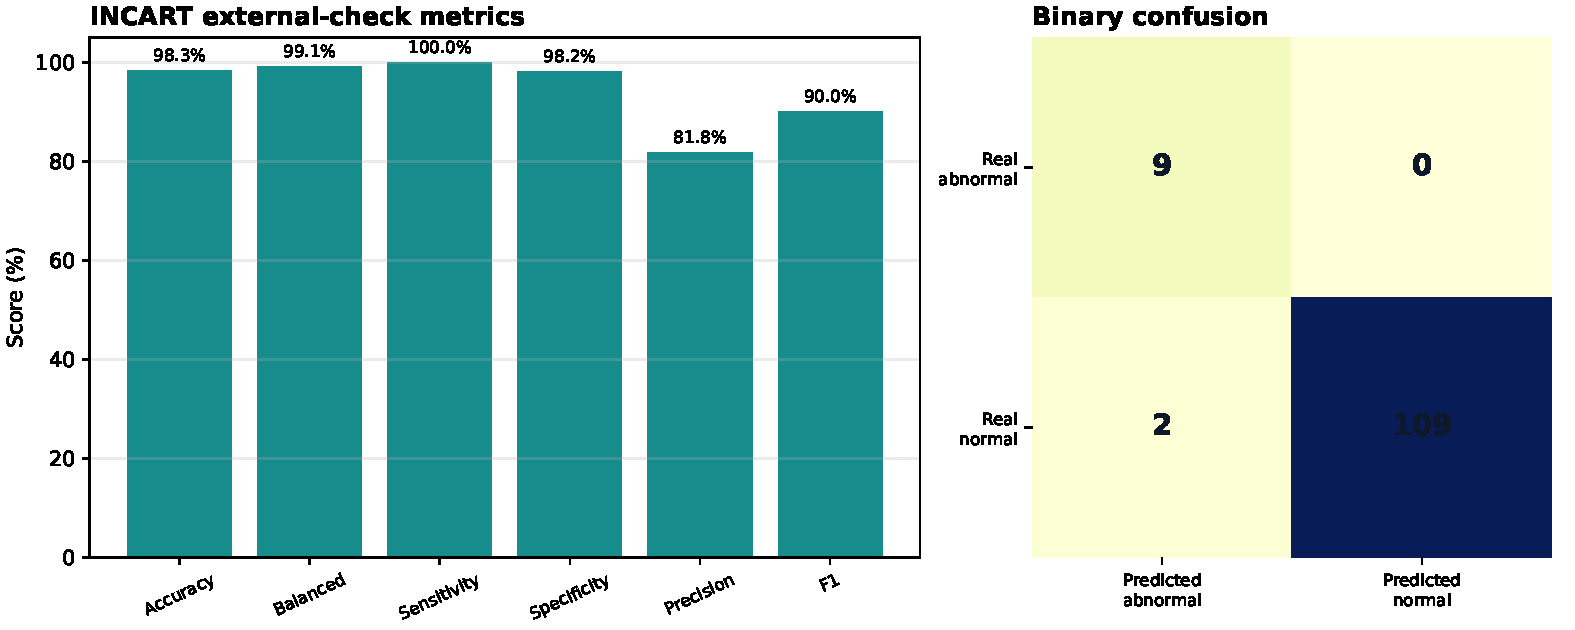
\includegraphics[width=.96\textwidth]{pic/generated/external_incart_metrics_confusion.pdf}
\caption{Metric bars and binary confusion matrix for the limited INCART
external check. Balanced accuracy is shown beside pooled accuracy because the
subset is class-imbalanced.}
\label{fig:external-incart-metrics}
\end{figure}

\begin{figure}[H]
\centering
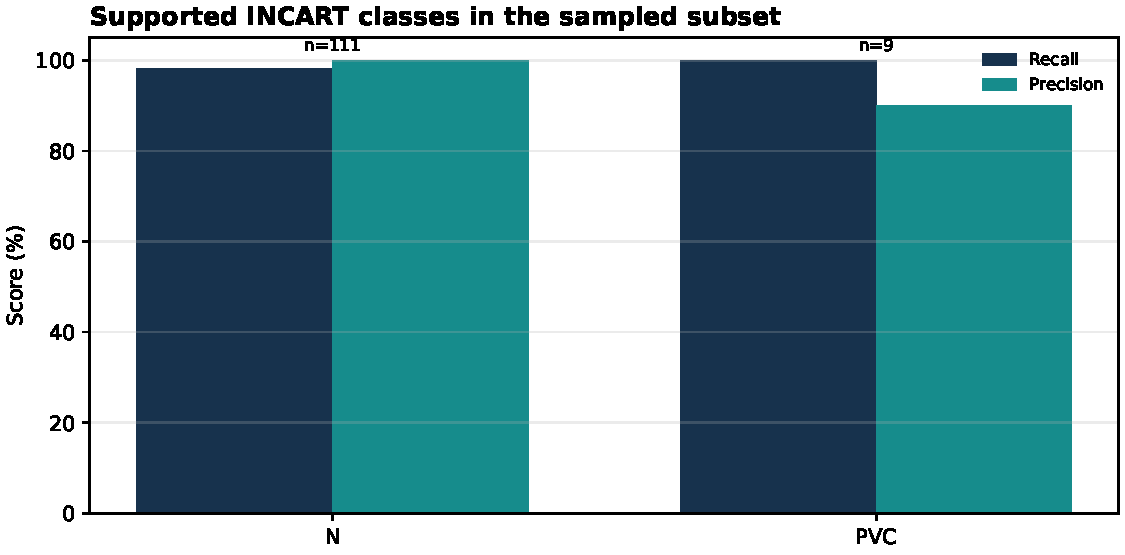
\includegraphics[width=.75\textwidth]{pic/generated/external_incart_class_summary.pdf}
\caption{Class-level precision and recall for classes that appear in the
limited INCART subset. Missing classes are not plotted because they have zero
support in this saved evaluation.}
\label{fig:external-incart-classes}
\end{figure}

\begin{table}[H]
\centering
\caption{Example annotated INCART beats used for visual inspection.}
\label{tab:external-incart-examples}
\begin{tabular}{rllll}
\toprule
No. & Record/sample & Real type & Predicted decision/type & Score\\
\midrule
1 & I01/353 & PVC (V) & Abnormal / PVC & 0.838\\
2 & I01/5426 & PVC (V) & Abnormal / PVC & 0.821\\
3 & I01/4253 & PVC (V) & Abnormal / PVC & 0.750\\
4 & I01/1322 & PVC (V) & Abnormal / PVC & 0.738\\
5 & I01/9029 & PVC (V) & Abnormal / PVC & 0.725\\
6 & I01/9430 & PVC (V) & Abnormal / PVC & 0.717\\
\bottomrule
\end{tabular}
\end{table}

\begin{figure}[H]
\centering
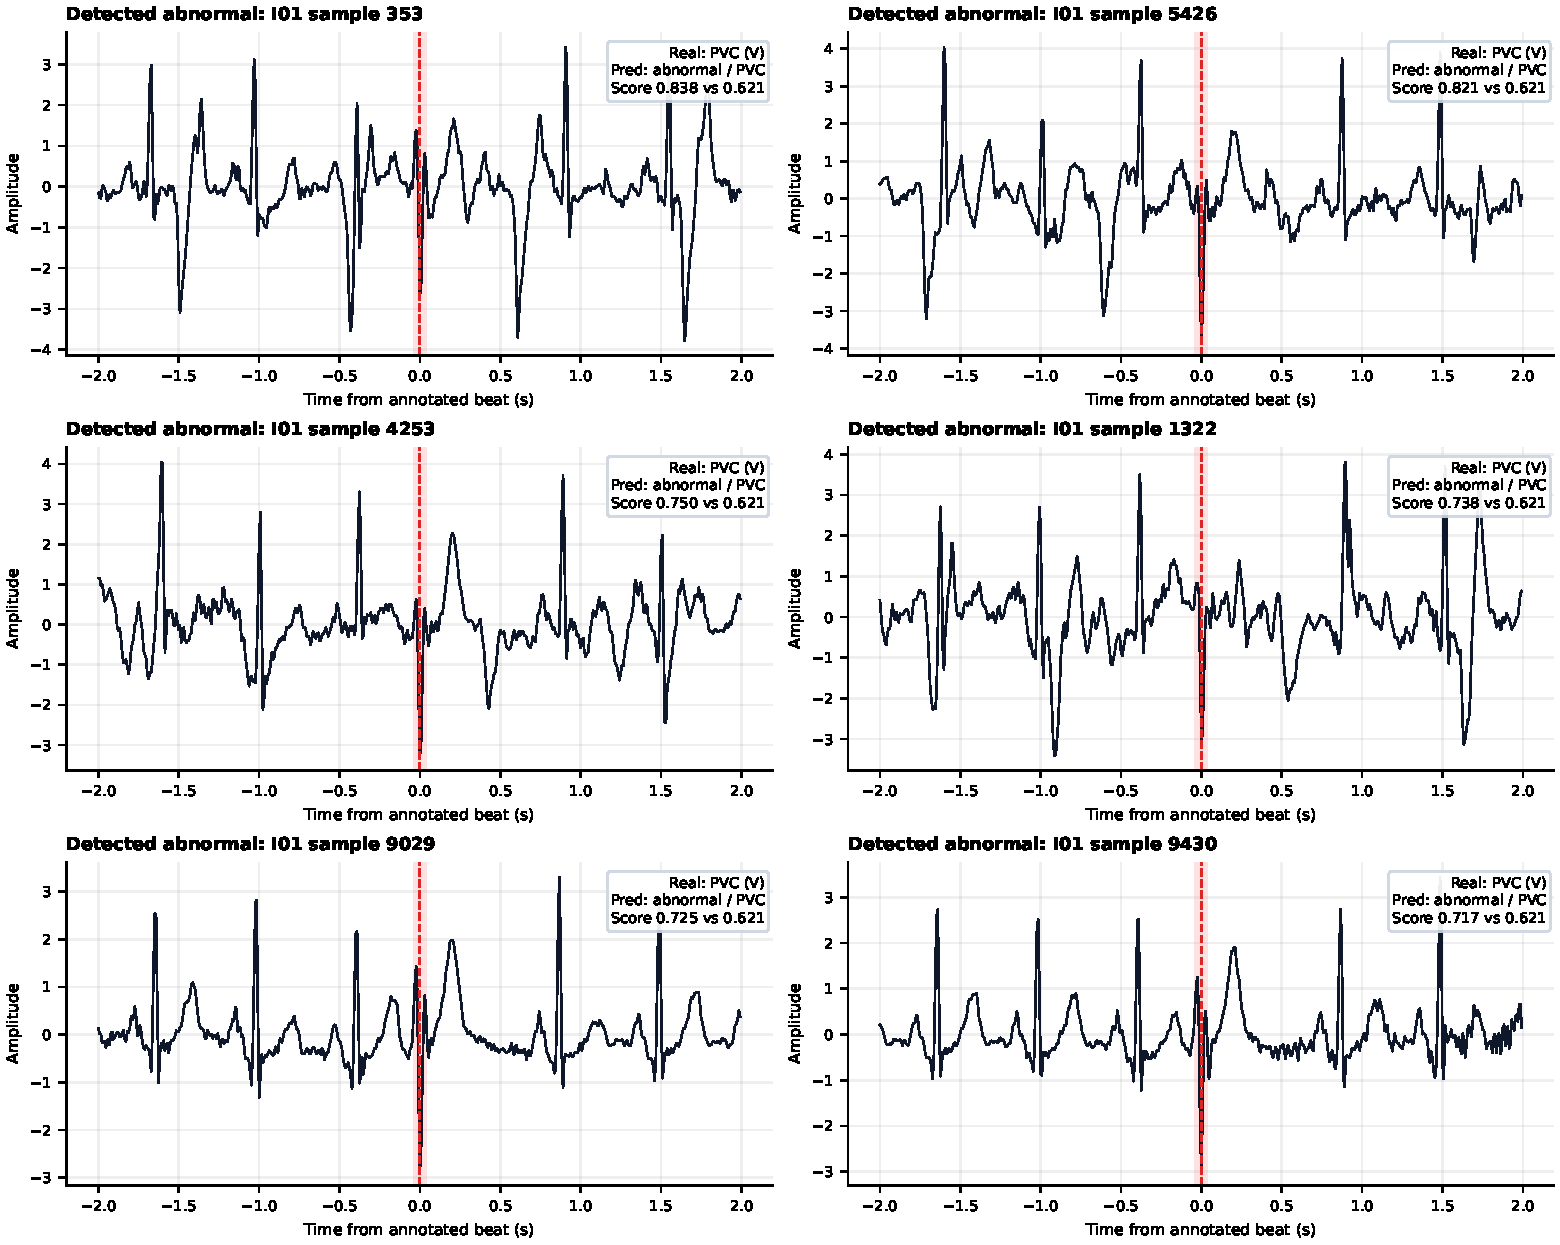
\includegraphics[width=.98\textwidth]{pic/generated/external_incart_examples.pdf}
\caption{Example INCART ECG segments centred on annotated beats. Each panel
shows the real annotation type, the model's abnormal/normal decision, the
predicted anomaly type, and the score-threshold comparison.}
\label{fig:external-incart-examples}
\end{figure}


\section{Answers to the research questions}

\begin{description}
    \item[RQ1] The frozen normal-only NSRDB autoencoder supplies four
    reconstruction-error features to both MLII supervised ensembles. A held-out
    ablation was not performed, so its independent contribution is not
    quantified.
    \item[RQ2] Abnormality detection reached 98.47\%, conditional subtype
    accuracy reached 95.20\%, and whole-system accuracy reached 96.86\% on the
    fixed temporal test.
    \item[RQ3] The whole-system equal-subject estimate was 96.90\%, with a
    94.02--99.05\% subject-clustered 95\% interval. Its lower bound is above
    90\%.
    \item[RQ4] The complete goal was not reached. The point estimate and lower
    confidence bound passed, but the interval width was 5.03 percentage points
    instead of at most three and PAC recall was 70.05\%. A limited post-freeze
    INCART external check was added in Section~\ref{sec:external-incart}, but
    it is too small to replace a full external clinical validation.
\end{description}
